\documentclass{standalone}
\usepackage{tikz}
\usetikzlibrary{calc}

\begin{document}
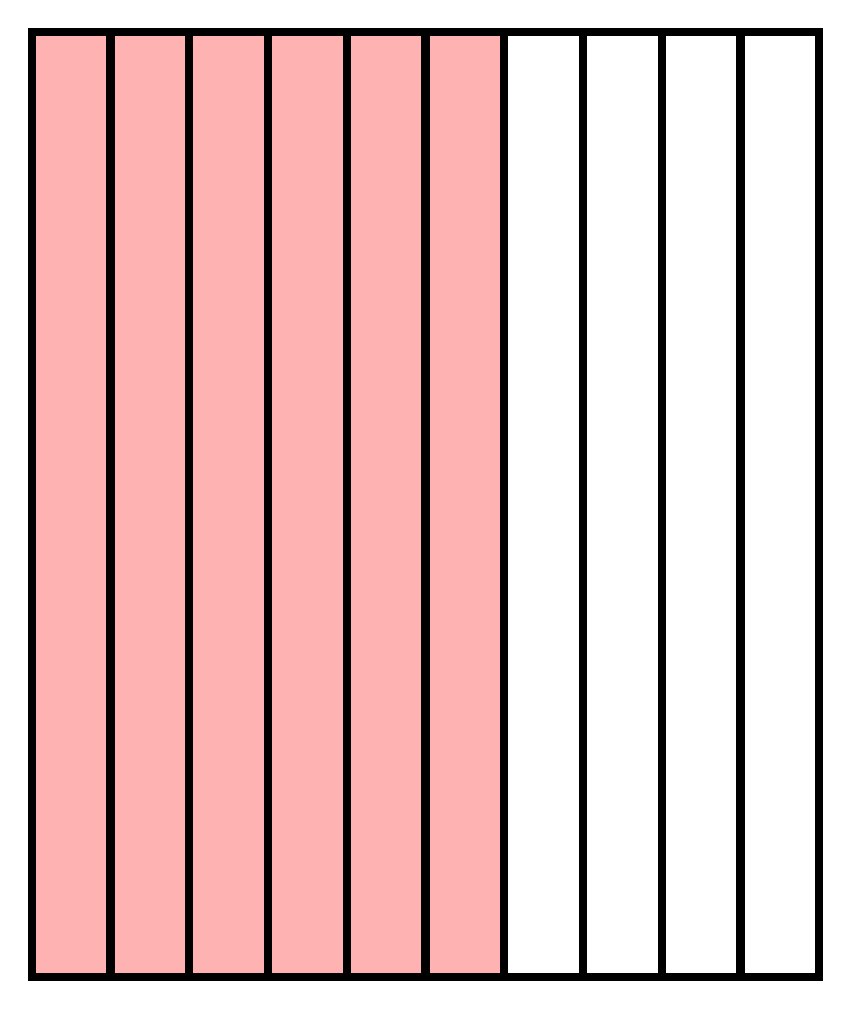
\begin{tikzpicture}

\coordinate (Center) at (0,0);
\coordinate (A1) at (-5,-6);
\coordinate (A2) at (-5,6);
\coordinate (A3) at (5,6);
\coordinate (A4) at (5,-6);
   
\fill[line width=3pt,color=red!30] (A1) rectangle ($(A2)!0.6!(A3)$); 

\draw[line width=3pt,color=black] (A1) rectangle ($(A2)!0.1!(A3)$); 
\draw[line width=3pt,color=black] (A1) rectangle ($(A2)!0.2!(A3)$); 
\draw[line width=3pt,color=black] (A1) rectangle ($(A2)!0.3!(A3)$); 
\draw[line width=3pt,color=black] (A1) rectangle ($(A2)!0.4!(A3)$); 
\draw[line width=3pt,color=black] (A1) rectangle ($(A2)!0.5!(A3)$); 
\draw[line width=3pt,color=black] (A1) rectangle ($(A2)!0.6!(A3)$); 
\draw[line width=3pt,color=black] (A1) rectangle ($(A2)!0.7!(A3)$); 
\draw[line width=3pt,color=black] (A1) rectangle ($(A2)!0.8!(A3)$); 
\draw[line width=3pt,color=black] (A1) rectangle ($(A2)!0.9!(A3)$); 
\draw[line width=3pt,color=black] (A1) rectangle (A3); 

\end{tikzpicture}

\end{document}